
%\RequirePackage{amsmath}
\documentclass[12pt]{article}

\usepackage{float}
\usepackage{multirow}
\newcommand{\ts}{\textsuperscript}
\usepackage{xcolor}
\usepackage{amssymb}
\definecolor{light-gray}{gray}{0.95}
\newcommand{\code}[1]{\colorbox{light-gray}{\texttt{#1}}}
\usepackage{graphicx}
\graphicspath{{plots/}}


\begin{document}



\title{
	%\logo{
%Computational Approach to School Geometry
	Sudoku Verifier
%	}
}
\author{ Rahul Ramachandran% <-this % stops a space
}

\date{\vspace{-4ex}}

\maketitle




\subsection{Graph 1}
The graph of time taken vs dimension of the sudoku (no. of threads is fixed at 16):
\begin{figure}[H]
    \centering
    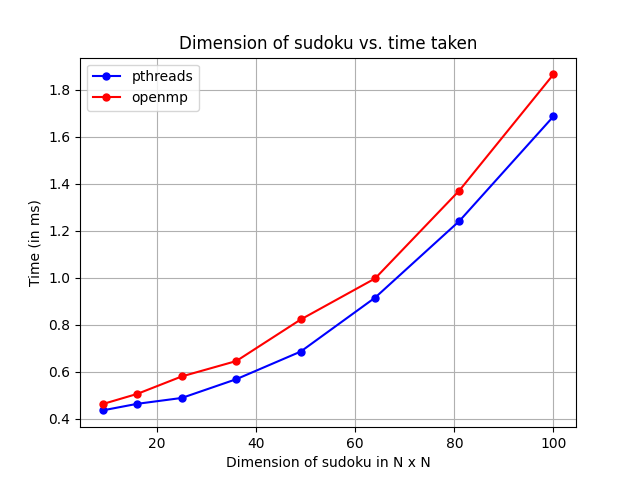
\includegraphics[width=\columnwidth]{Figure_1.png}
    \caption{time taken vs dimension of the sudoku}
    \label{fig-1}
  \end{figure}

Since the number of threads is fixed, and since checking the validity of the sudoku has a 
time complexity of $O(n^2)$, we expect a quadratic curve, which is what is observed.
A second observation is that OpenMP is slightly slower than pthreads. This is because OpenMP
is a higher level API, and is optimised for ease of use over performance. On the otherhand, pthreads
offers more flexibility and is lower-level, and therefore consistently (but narrowly) beats OpenMP.


\subsection{Graph 2}
The graph of time taken vs no. of threads (dimension of sudoku is fixed at 25x25):
\begin{figure}[H]
    \centering
    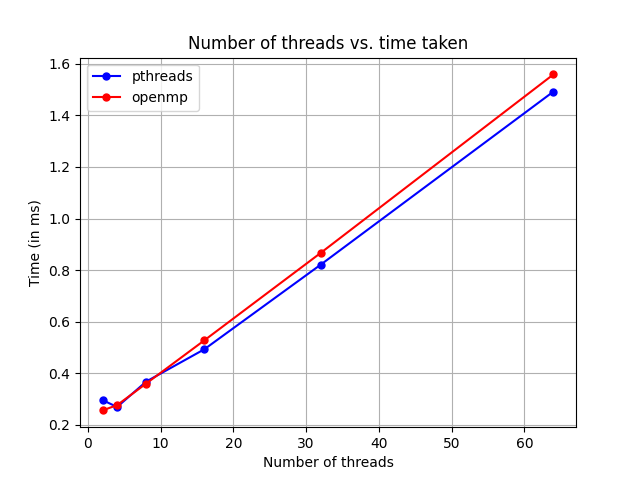
\includegraphics[width=\columnwidth]{Figure_2.png}
    \caption{time taken vs no. of threads}
    \label{fig-2}
  \end{figure}

While we would usually expect the time to decrease with the number of threads, it is observed
that the time actually increases. This happens for a number of reasons:
\begin{itemize}
    \item By Amdahl's Law, the speedup is $ <= \frac{1}{S+\frac{1-S}{N}}$, where $S$ is the fraction of serial code. In other words, as the nummber of threads increases, the serial portion of the code becomes the bottleneck, as the speedup will always be $<= \frac{1}{S}$. Note that because of the 
    small input size here, there isn't much scope for parallelization. 
    \item Since there is an inherent limit to the multithreading capability of a system (by the number of cores), increasing the number of threads beyond a point will not help reduce the time taken. (The number of cores in the system used to run the code is 4)
    \item   After a point, thread overheads (like context-switching between many threads for instance) become significant, and outweigh the speedup gained due to multithreading.
\end{itemize}

When the code is run for a much larger dimension (egs: 10000x10000), a decrease \emph{is} observed (though for a large number of threads, the time still increases due to the above
factors). As before, we note that the execution is faster for pthreads than OpenMP. The plot linearly increases with the number of threads, hinting toward a constant overhead time
per thread created.


\end{document}